% Standalone TikZ for Figure 2: SPI Arbiter State Machine (clean, no overlap)
\documentclass[border=15pt]{standalone}
\usepackage{tikz}
\usetikzlibrary{shapes.geometric, positioning, arrows.meta, calc, fit}
\definecolor{vbfcBlue}{HTML}{1B4F72}
\definecolor{vbfcDarkBlue}{HTML}{0D2B40}
\definecolor{vbfcAccent}{HTML}{E86C00}
\definecolor{vbfcLightGray}{HTML}{F2F2F2}
\definecolor{vbfcMediumGray}{HTML}{CCCCCC}
\definecolor{vbfcDarkGray}{HTML}{555555}
\definecolor{vbfcOrange}{HTML}{F39C12}
\definecolor{vbfcGreen}{HTML}{27AE60}
\definecolor{vbfcRed}{HTML}{C0392B}
\definecolor{vbfcTeal}{HTML}{16A085}
\definecolor{vbfcPurple}{HTML}{8E44AD}
\begin{document}
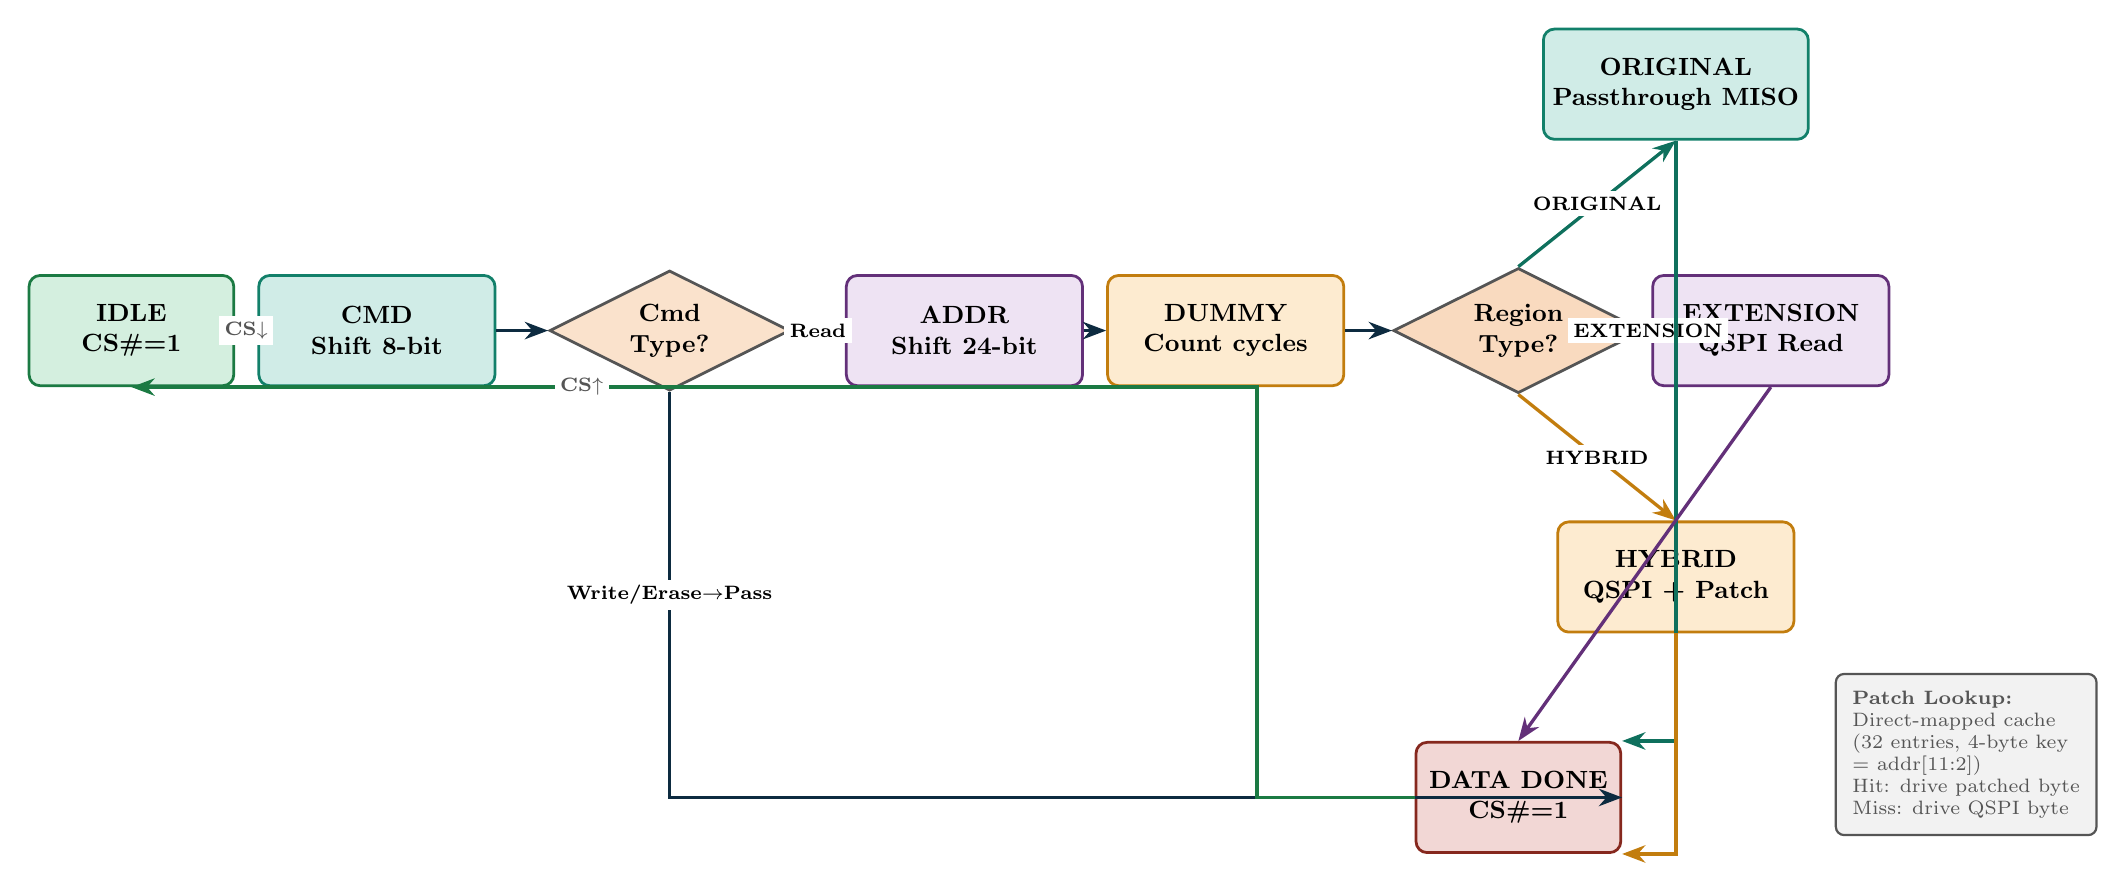
\begin{tikzpicture}[
    node distance=12mm,
    state/.style={
        draw=vbfcDarkBlue, line width=1pt, rounded corners=4pt,
        fill=vbfcBlue!12, minimum height=14mm, minimum width=30mm,
        align=center, font=\small, font=\bfseries\small
    },
    decst/.style={
        draw=vbfcDarkGray, line width=1pt, diamond, aspect=2,
        fill=vbfcAccent!20, minimum height=10mm, minimum width=26mm,
        align=center, font=\small\bfseries
    },
    startst/.style={
        draw=vbfcGreen!70!black, line width=1pt, rounded corners=4pt,
        fill=vbfcGreen!20, minimum height=14mm, minimum width=26mm,
        align=center, font=\bfseries\small
    },
    endst/.style={
        draw=vbfcRed!70!black, line width=1pt, rounded corners=4pt,
        fill=vbfcRed!20, minimum height=14mm, minimum width=26mm,
        align=center, font=\bfseries\small
    },
    arrow/.style={-Stealth, line width=1.2pt, draw=vbfcDarkBlue},
    origarrow/.style={-Stealth, line width=1.2pt, draw=vbfcTeal!70!black},
    extarrow/.style={-Stealth, line width=1.2pt, draw=vbfcPurple!70!black},
    hybarrow/.style={-Stealth, line width=1.2pt, draw=vbfcOrange!80!black},
    labelstyle/.style={font=\scriptsize\bfseries, text=vbfcDarkGray, fill=white, inner sep=2pt},
    ellabel/.style={font=\scriptsize\bfseries, fill=white, inner sep=2pt}
]

% Row 1: IDLE → CMD → CMD_DEC  → ADDR → DUMMY → ROUTE
\node[startst] (idle) {IDLE\\CS\#=1};
\node[state, fill=vbfcTeal!20, draw=vbfcTeal!80!black] (cmd) at ($(idle.east)+(18mm,0)$) {CMD\\Shift 8-bit};
\node[decst] (cmd_dec) at ($(cmd.east)+(22mm,0)$) {Cmd\\Type?};
\node[state, fill=vbfcPurple!15, draw=vbfcPurple!70!black] (addr) at ($(cmd_dec.east)+(22mm,0)$) {ADDR\\Shift 24-bit};
\node[state, fill=vbfcOrange!20, draw=vbfcOrange!80!black] (dummy) at ($(addr.east)+(18mm,0)$) {DUMMY\\Count cycles};
\node[decst, fill=vbfcAccent!25] (route) at ($(dummy.east)+(22mm,0)$) {Region\\Type?};

% Row 2: Branches from ROUTE
\node[state, fill=vbfcTeal!20, draw=vbfcTeal!80!black, anchor=south] (orig) at ($(route.north)+(20mm,16mm)$) {ORIGINAL\\Passthrough MISO};
\node[state, fill=vbfcPurple!15, draw=vbfcPurple!70!black] (ext) at ($(route.east)+(16mm,0)$) {EXTENSION\\QSPI Read};
\node[state, fill=vbfcOrange!20, draw=vbfcOrange!80!black, anchor=north] (hybrid) at ($(route.south)+(20mm,-16mm)$) {HYBRID\\QSPI + Patch};

% DONE state
\node[endst, anchor=north] (done) at ($(route.south)+(0mm,-44mm)$) {DATA DONE\\CS\#=1};

% Arrows row 1
\draw[arrow] (idle) -- node[labelstyle] {CS$\downarrow$} (cmd);
\draw[arrow] (cmd) -- (cmd_dec);
\draw[arrow] (cmd_dec) -- node[ellabel, sloped] {Read} (addr);
% Write/Erase bypass
\draw[arrow] (cmd_dec.south) |- node[ellabel, pos=0.25] {Write/Erase$\to$Pass} (done.east);
\draw[arrow] (addr) -- (dummy);
\draw[arrow] (dummy) -- (route);

% Branch arrows
\draw[origarrow] (route.north) -- node[ellabel] {ORIGINAL} (orig.south);
\draw[extarrow] (route.east) -- node[ellabel] {EXTENSION} (ext.west);
\draw[hybarrow] (route.south) -- node[ellabel] {HYBRID} (hybrid.north);

% To DONE
\draw[origarrow] (orig.south) |- (done.north east);
\draw[extarrow] (ext.south) -- (done.north);
\draw[hybarrow] (hybrid.south) |- (done.south east);

% DONE → IDLE (back)
\draw[arrow, draw=vbfcGreen!70!black] (done.west) -- ++(-20mm,0) |- node[labelstyle, pos=0.8] {CS$\uparrow$} (idle.south);

% Patch cache info box
\node[draw=vbfcDarkGray, line width=0.8pt, rounded corners=3pt, fill=vbfcLightGray,
      font=\scriptsize, text=vbfcDarkGray, anchor=north west, inner sep=6pt, align=left] at ($(hybrid.south east)+(5mm,-5mm)$) {
    \textbf{Patch Lookup:}\\
    Direct-mapped cache\\
    (32 entries, 4-byte key\\
    = addr[11:2])\\
    Hit: drive patched byte\\
    Miss: drive QSPI byte
};

\end{tikzpicture}
\end{document}
